% !TeX root = thesis.tex
%--------------------------------------------------------------------%
%
% Templat LaTeX Laporan Tugas Akhir Non-Konvensional
% BENTUK 2: PROYEK KELOMPOK BERSAMA MITRA (CAPSTONE)
% Program Studi Teknik Informatika ITERA
%
% Disusun ulang dari "Templat_Laporan_TA_Bentuk2_Proyek_Capstone" (Word)
% di atas templat LaTeX TA IF ITERA versi 2026.1 (format UNESCO).
% Berkas format lama disimpan di chapters/arsip-format-lama/ dan tidak
% ikut dikompilasi.
%
%--------------------------------------------------------------------%

% Ukuran naskah UNESCO 15,5 x 23 cm, Times New Roman 11 pt
\documentclass[11pt]{report}
\usepackage[paperwidth=155mm,
			paperheight=230mm,
			top=2cm,
			bottom=2cm,
			left=2cm,
			right=2cm,
			includefoot,
			heightrounded,
			bindingoffset=0.5cm]   % margin sisi jilid = 2 + 0,5 = 2,5 cm
			{geometry}

\input{config/config.sty}   % Konfigurasi templat ITERA
%-------------------------------------------------------------------%
% Pengaturan tambahan untuk Templat Laporan TA Bentuk 2
% (Proyek Kelompok bersama Mitra / Capstone), Prodi IF ITERA.
% Dipanggil dari thesis.tex setelah config/config.sty.
%-------------------------------------------------------------------%
\usepackage{colortbl}
\usepackage{amssymb}
\usepackage{pdfpages}

%----- Judul bab: satu baris, tengah, tebal, huruf kapital ---------%
% Contoh: "BAB I MASALAH MITRA DAN TUJUAN PROYEK"
\titleformat{\chapter}[block]%
  {\large\centering\bfseries}%
  {\MakeUppercase{\chaptertitlename}\ \thechapter}{0.4em}%
  {\MakeUppercase}
\titlespacing*{\chapter}{0pt}{0pt}{12pt}

%----- Nomor halaman: tengah bawah pada semua halaman --------------%
\fancypagestyle{capstone}{%
  \fancyhf{}%
  \renewcommand{\headrulewidth}{0pt}%
  \fancyfoot[C]{\thepage}%
}
\fancypagestyle{plain}{%
  \fancyhf{}%
  \renewcommand{\headrulewidth}{0pt}%
  \fancyfoot[C]{\thepage}%
}

%----- Saklar petunjuk ---------------------------------------------%
% \petunjuktrue  = teks "Petunjuk:" dan halaman Petunjuk Pengisian
%                  serta Peta Kewajiban DITAMPILKAN (saat menulis).
% \petunjukfalse = semua petunjuk DISEMBUNYIKAN (naskah final).
\newif\ifpetunjuk
\petunjuktrue

%----- Penanda status kewajiban ------------------------------------%
\newcommand{\wajib}[1]{\textcolor{red!75!black}{\textbf{\upshape #1}}}
\newcommand{\opsional}[1]{\colorbox{yellow!55}{\textbf{\upshape #1}}}
\newcommand{\tidakperlu}[1]{\textcolor{gray}{\upshape #1}}
% [Seminar proposal: ... · Sidang akhir: ...]
\newcommand{\tahap}[2]{[Seminar proposal: #1 $\cdot$ Sidang akhir: #2]}

%----- Kotak petunjuk (miring, abu-abu, spasi 1) -------------------%
\newcommand{\petunjuk}[1]{%
  \ifpetunjuk
    \par\begingroup\setlength{\parindent}{0pt}\singlespacing\footnotesize\itshape
    \textcolor{gray!60!black}{\textbf{Petunjuk:} #1}\par\endgroup\vspace{4pt}%
  \fi}

%----- Teks isian (abu-abu dalam kurung siku) ----------------------%
\newcommand{\isian}[1]{\textcolor{gray}{[#1]}}
\newcommand{\tulisuraian}{\par\textcolor{gray}{[Tulis uraian dalam bentuk paragraf.]}\par}

%----- Judul halaman tanpa nomor yang masuk daftar isi -------------%
% Contoh: \judulhalaman{KATA PENGANTAR}
\newcommand{\judulhalaman}[1]{%
  \chapter*{#1}%
  \phantomsection\addcontentsline{toc}{chapter}{#1}%
  \thispagestyle{capstone}}

%----- Subbab tanpa nomor otomatis (P.3.1, dst.) --------------------%
\newcommand{\subbabP}[1]{%
  \section*{#1}%
  \phantomsection\addcontentsline{toc}{section}{#1}}

%----- Halaman pembatas BAGIAN I / BAGIAN II -----------------------%
\newcommand{\halamanbagian}[2]{%
  \chapter*{#1}%
  \phantomsection\addcontentsline{toc}{chapter}{#1}%
  \thispagestyle{capstone}%
  {\centering\itshape #2\par}}

%----- Sel tabel berwarna untuk Peta Kewajiban ---------------------%
\newcommand{\cW}[1]{\cellcolor{red!12}\textcolor{red!75!black}{\textbf{#1}}}
\newcommand{\cO}[1]{\cellcolor{yellow!35}\textbf{#1}}
\newcommand{\cT}[1]{\cellcolor{gray!15}\textcolor{gray!80!black}{#1}}
\newcommand{\cekbox}{$\square$}

%----- Variabel informasi laporan ----------------------------------%
\makeatletter
\newcommand{\proyekTim}[1]{\def\@proyektim{#1}}
\newcommand{\printproyektim}{\@proyektim}
\newcommand{\anggotaLain}[1]{\def\@anggotalain{#1}}
\newcommand{\printanggotalain}{\@anggotalain}
\newcommand{\namaMitra}[1]{\def\@namamitra{#1}}
\newcommand{\printnamamitra}{\@namamitra}
\newcommand{\tempatLahir}[1]{\def\@tempatlahir{#1}}
\newcommand{\printtempatlahir}{\@tempatlahir}
\newcommand{\tahunLaporan}[1]{\def\@tahunlaporan{#1}}
\newcommand{\printtahunlaporan}{\@tahunlaporan}
\newcommand{\tanggalLaporan}[1]{\def\@tanggallaporan{#1}}
\newcommand{\printtanggallaporan}{\@tanggallaporan}
\newcommand{\koordinatorProdi}[2]{\def\@namakoor{#1}\def\@nipkoor{#2}}
\newcommand{\printnamakoor}{\@namakoor}
\newcommand{\printnipkoor}{\@nipkoor}
\makeatother
 % Tambahan khusus templat capstone

% TIPS OVERLEAF GRATIS (batas waktu kompilasi):
% aktifkan baris di bawah agar hanya bab yang sedang dikerjakan yang
% dikompilasi. Nonaktifkan lagi sebelum mengompilasi dokumen lengkap.
% \includeonly{chapters/bab-1}

%--------------------------------------------------------------------%
% SAKLAR PETUNJUK
% \petunjuktrue  : teks "Petunjuk:", halaman Petunjuk Pengisian, dan
%                  Peta Kewajiban ditampilkan (saat menulis).
% \petunjukfalse : semuanya disembunyikan (naskah yang diserahkan).
%--------------------------------------------------------------------%
\petunjuktrue

\begin{document}

    %----------------------------------------------------------------%
    % INFORMASI LAPORAN (ubah di sini, otomatis dipakai di semua halaman)
    %----------------------------------------------------------------%
    % Judul Laporan TA individu (maks. 16 kata, beda dari anggota lain)
    \title{Rancang Bangun Permissioned Blockchain dan Smart Contract Multi-Otoritas untuk Surat Keterangan Lulus (Studi Kasus: SMAN 1 Gadingrejo)}
    \titleEN{[Judul dalam bahasa Inggris]}

    \author{Doni Agus Setiawan}             % Nama mahasiswa
    \nim{123140009}                         % NIM
    \tempatLahir{[Tempat, tanggal lahir]}   % untuk Pernyataan Orisinalitas

    \proyekTim{Sistem Verifikasi Dokumen Akademik Siswa pada Sekolah Menengah Atas Berbasis Permissioned Blockchain dan Smart Contract Multi-Otoritas}
    \anggotaLain{[Nama dan NIM anggota 2]; [Nama dan NIM anggota 3]; [Nama dan NIM anggota 4]}
    \namaMitra{SMAN 1 Gadingrejo}

    % Pembimbing (templat capstone: satu pembimbing)
    \dosbingA{[Nama dan gelar pembimbing]}{NIP. [..................]}
    % Penguji
    \pengujiA{[Nama dan gelar penguji 1]}{NIP. [..................]}
    \pengujiB{[Nama dan gelar penguji 2]}{NIP. [..................]}
    % Koordinator Program Studi
    \koordinatorProdi{Andika Setiawan, S.Kom., M.Cs.}{NIP. 19911127 2022 03 1 007}

    \tanggalLaporan{[tanggal]}   % contoh: 20 November 2026
    \tahunLaporan{2026}

	\sloppy
    \pagenumbering{roman}
    \setcounter{page}{1}

	%----------------------------------------------------------------%
	% HALAMAN AWAL
	%----------------------------------------------------------------%
	%--------------------------------------------------------------------%
% SAMPUL
%--------------------------------------------------------------------%
\clearpage
\thispagestyle{empty}
\begin{center}
	\singlespacing
	\vspace*{0.3cm}
	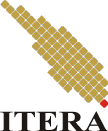
\includegraphics[height=1.9cm]{figure/logo-itera-kiri.png}\hspace{1pt}%
	
\includegraphics[height=1.55cm]{figure/logo-itera-kanan.png}\hspace{1.2cm}%
	
\includegraphics[height=1.55cm]{figure/logo-diktisaintek-berdampak.png}

	\vspace{1cm}
	{\bfseries TUGAS AKHIR NON-KONVENSIONAL\\
	\large LAPORAN PROYEK (CAPSTONE)\\}
	{\normalsize Bentuk 2: Proyek Kelompok bersama Mitra}

	\vspace{0.7cm}
	{\large\bfseries \MakeUppercase{\thetitle}\par}
	\vspace{0.6cm}
	Diajukan sebagai luaran mata kuliah Tugas Akhir (IF25-40033)

	\vspace{0.8cm}
	\textbf{Disusun oleh:}\\[2pt]
	\theauthor\quad \printnim\\
	Proyek tim: \printproyektim\\
	Anggota tim lain: \printanggotalain

	\vspace{0.5cm}
	Pembimbing: \printnamadosbinga\\
	Mitra: \printnamamitra

	\vfill
	{\bfseries PROGRAM STUDI TEKNIK INFORMATIKA\\
	FAKULTAS TEKNOLOGI INDUSTRI\\
	INSTITUT TEKNOLOGI SUMATERA\\
	LAMPUNG SELATAN\\
	\printtahunlaporan}
	\vspace*{0.5cm}
\end{center}
\clearpage
            % Sampul
	%--------------------------------------------------------------------%
% LEMBAR PENGESAHAN
%--------------------------------------------------------------------%
\clearpage
\setcounter{page}{2}
\judulhalaman{LEMBAR PENGESAHAN}
\begingroup
\singlespacing\setlength{\parindent}{0pt}
Saya menyatakan bahwa Tugas Akhir berjudul ``\thetitle'' merupakan hasil karya saya sendiri dan belum pernah diajukan, baik sebagian maupun seluruhnya, di Institut Teknologi Sumatera atau institusi pendidikan lain oleh saya maupun pihak lain.

\vspace{0.3cm}
\begin{tabular}{@{}p{0.62\textwidth}@{}p{0.36\textwidth}@{}}
	Lampung Selatan, \printtanggallaporan & \multirow{5}{*}{\hfill\fbox{\parbox[c][3.2cm][c]{2.4cm}{\centering\footnotesize Pas foto 3$\times$4\\berwarna}}}\\
	& \\
	& \\
	\theauthor & \\
	\printnim & \\
\end{tabular}

\vspace{0.3cm}
Diperiksa dan disetujui oleh,\\[4pt]
Pembimbing\\
\hspace*{1em}1. \printnamadosbinga\\
\hspace*{1.9em}\printnipdosbinga\\[4pt]
Penguji\\
\hspace*{1em}1. \printnamapengujia\\
\hspace*{1.9em}\printnippengujia\\
\hspace*{1em}2. \printnamapengujib\\
\hspace*{1.9em}\printnippengujib

\vspace{0.2cm}
\vspace*{-\topsep}\begin{center}
	Disahkan oleh,\\
	Koordinator Program Studi Teknik Informatika\\
	Fakultas Teknologi Industri\\
	Institut Teknologi Sumatera\\[1.3cm]
	\printnamakoor\\
	\printnipkoor
\end{center}
\endgroup
\clearpage
         % Lembar Pengesahan (hal. ii)
    \clearpage
	\newgeometry{top=2cm, bottom=2cm, left=2cm, right=2cm,
		includefoot, heightrounded, bindingoffset=0.5cm,
		twoside}                      % cetak bolak-balik, margin cermin
    \pagestyle{capstone}
	%--------------------------------------------------------------------%
% HALAMAN PERNYATAAN ORISINALITAS
%--------------------------------------------------------------------%
\judulhalaman{HALAMAN PERNYATAAN ORISINALITAS}
\begingroup
\setlength{\parindent}{0pt}
Yang bertanda tangan di bawah ini:

\begin{tabular}{@{}l@{\ }l@{\ }p{0.62\textwidth}@{}}
	Nama & : & \theauthor\\
	NIM & : & \printnim\\
	Tempat, tgl. lahir & : & \printtempatlahir\\
	Program studi & : & Teknik Informatika\\
	Fakultas & : & Teknologi Industri\\
	Judul Laporan TA & : & \thetitle\\
\end{tabular}

menyatakan dengan sesungguhnya bahwa:
\begin{enumerate}
	\item Laporan Tugas Akhir dengan judul tersebut adalah hasil karya saya sendiri yang membahas bagian proyek yang menjadi tanggung jawab saya sesuai Surat Pembagian Kerja Tim, bukan duplikasi atau plagiasi dari karya orang lain, dan belum pernah diajukan untuk memperoleh gelar kesarjanaan di perguruan tinggi mana pun.
	\item Bagian konteks proyek (profil dan masalah mitra, gambaran dan arsitektur umum, serta tinjauan pustaka bersama) dapat beririsan dengan laporan anggota tim lain; tujuan, rancangan, implementasi, pengujian, pembahasan, dan kesimpulan bagian saya ditulis sendiri (Pedoman TA 5.1.3).
	\item Laporan ini tidak mengandung fabrikasi maupun falsifikasi data pengujian, dan seluruh sumber yang dikutip maupun dirujuk telah saya nyatakan dengan benar.
	\item \textit{Logbook} dan \textit{peer assessment} saya isi dengan jujur sesuai kontribusi saya yang sebenarnya.
	\item Data dan dokumen mitra saya pakai dengan izin mitra dan kerahasiaannya dijaga.
	\item Penggunaan AI generatif, bila ada, telah saya nyatakan secara jujur pada Halaman Pernyataan Penggunaan AI.
\end{enumerate}

Apabila di kemudian hari terbukti terdapat penyimpangan atau ketidakbenaran dalam pernyataan ini, saya bersedia menerima sanksi akademik sesuai dengan peraturan yang berlaku di Institut Teknologi Sumatera, termasuk pencabutan gelar kesarjanaan yang telah saya peroleh.

\vspace{0.4cm}
Lampung Selatan, \printtanggallaporan

\begin{flushright}
	\begin{minipage}{0.45\textwidth}\centering\singlespacing
		Yang membuat pernyataan,\\[0.6cm]
		\textcolor{gray}{[Materai Rp10.000]}\\[0.6cm]
		(\theauthor)\\
		NIM. \printnim
	\end{minipage}
\end{flushright}
\endgroup
\clearpage
        % Pernyataan Orisinalitas
	%--------------------------------------------------------------------%
% HALAMAN PERNYATAAN PENGGUNAAN KECERDASAN ARTIFISIAL (AI)
% Seminar proposal: Tidak diperlukan . Sidang akhir: WAJIB
% Untuk seminar proposal, halaman ini boleh dinonaktifkan di thesis.tex.
%--------------------------------------------------------------------%
\judulhalaman{HALAMAN PERNYATAAN PENGGUNAAN KECERDASAN ARTIFISIAL (AI)}
\petunjuk{Wajib diisi pada laporan sidang akhir, termasuk bila tidak memakai AI (Pedoman TA Bab 4.2.1, Lampiran 2). Untuk TA kelompok, setiap anggota mengisi satu halaman ini. Lampirkan log sesi AI dan riwayat versi laporan serta kode. \tahap{\tidakperlu{Tidak diperlukan}}{\wajib{WAJIB}}}
\begingroup
\setlength{\parindent}{0pt}
Yang bertanda tangan di bawah ini:

\begin{tabular}{@{}l@{\ }l@{\ }p{0.62\textwidth}@{}}
	Nama & : & \theauthor\\
	NIM & : & \printnim\\
	Program studi & : & Teknik Informatika\\
	Judul Tugas Akhir & : & \thetitle\\
\end{tabular}

menyatakan dengan sesungguhnya bahwa dalam proses penyusunan Tugas Akhir ini, saya:

\cekbox\ \textbf{TIDAK} menggunakan alat bantu Kecerdasan Artifisial (AI) dalam bentuk apa pun.

\cekbox\ \textbf{MENGGUNAKAN} alat bantu Kecerdasan Artifisial (AI) dengan rincian pada tabel berikut.

{\singlespacing\footnotesize
\begin{center}
\begin{tabular}{|p{0.06\textwidth}|p{0.2\textwidth}|p{0.18\textwidth}|p{0.18\textwidth}|p{0.18\textwidth}|}
	\hline
	\textbf{No} & \textbf{Nama AI dan versi} & \textbf{Tujuan} & \textbf{Bagian TA} & \textbf{Verifikasi}\\ \hline
	1 & & & & \\[8pt] \hline
	2 & & & & \\[8pt] \hline
	3 & & & & \\[8pt] \hline
\end{tabular}
\end{center}}

Saya menyadari dan bertanggung jawab penuh bahwa:
\begin{enumerate}
	\item Seluruh isi Tugas Akhir, termasuk bagian yang dibantu AI, merupakan tanggung jawab saya sepenuhnya.
	\item Setiap fakta, referensi, dan data yang diperoleh dari AI telah saya verifikasi kebenarannya.
	\item Saya mampu menjelaskan seluruh bagian Tugas Akhir secara lisan, termasuk \textit{code walkthrough}.
	\item Apabila ditemukan ketidakjujuran dalam pernyataan ini, saya bersedia menerima sanksi akademik sesuai Peraturan Rektor ITERA Nomor 10 Tahun 2025.
\end{enumerate}

\begin{flushright}
	\begin{minipage}{0.45\textwidth}\centering\singlespacing
		Lampung Selatan, \printtanggallaporan\\
		Yang membuat pernyataan,\\[1.4cm]
		(\theauthor)\\
		NIM. \printnim
	\end{minipage}
\end{flushright}
\endgroup
\clearpage
     % Pernyataan Penggunaan AI (WAJIB sidang akhir)
	\ifpetunjuk
		%--------------------------------------------------------------------%
% PETUNJUK PENGISIAN
% Halaman ini otomatis hilang bila \petunjukfalse di thesis.tex.
%--------------------------------------------------------------------%
\chapter*{PETUNJUK PENGISIAN}
\thispagestyle{capstone}
{\itshape Halaman ini dan halaman Peta Kewajiban dihapus dari naskah final (atur \texttt{\textbackslash petunjukfalse} di \texttt{thesis.tex}). Isi setiap bab dan subbab dalam bentuk paragraf. Teks miring berawalan ``Petunjuk:'' menjelaskan isi yang diharapkan dan otomatis hilang saat saklar petunjuk dimatikan; teks abu-abu dalam kurung siku diganti dengan isi Anda.

Tabel hanya dipakai untuk menyajikan data yang memang berbentuk tabel, diberi nomor dan judul (Tabel 2.1 di atas tabel), dan dirujuk dalam narasi. Jangan menulis isi bab atau subbab di dalam tabel atau kotak.\par}

\begin{itemize}
	\item Judul penelitian maksimal 16 kata dan ditulis sama persis di sampul, lembar pengesahan, pernyataan, dan presentasi.
	\item Ukuran naskah UNESCO (lebar 15,5 cm $\times$ tinggi 23 cm), Times New Roman 11 pt, spasi 1,5 (spasi 1 untuk abstrak, isi tabel, dan daftar pustaka), rata kiri-kanan (\textit{justify}). Margin atas 2 cm, kiri 2,5 cm, bawah 2 cm, kanan 2 cm; dicetak bolak-balik dengan margin cermin (margin 2,5 cm selalu di sisi jilid).
	\item Setiap anggota menyusun Laporan TA individu atas namanya sendiri dengan judul berbeda, membahas bagian proyek yang menjadi tanggung jawabnya (Pedoman TA 5.1.3). Bagian konteks proyek (profil dan masalah mitra, gambaran dan arsitektur umum, tinjauan pustaka bersama) boleh sama antaranggota; tujuan, rancangan, implementasi, pengujian, pembahasan, dan kesimpulan bagian individu wajib ditulis sendiri. Judul laporan individu ditetapkan saat seminar proposal dan dicantumkan dalam Surat Pembagian Kerja Tim.
	\item Proyek dikerjakan kelompok 3 sampai 4 mahasiswa bersama mitra berbadan hukum. Tiap anggota menyimpan \textit{logbook} individu dan mengisi \textit{peer assessment} sendiri secara rahasia; evaluasi kontribusi oleh pembimbing diisi terpisah (Pedoman TA butir 3.3.2 dan 3.3.4).
	\item Proyek dikerjakan kelompok 3 sampai 4 mahasiswa (lebih dari 4 dengan persetujuan Kaprodi) bersama mitra berbadan hukum, dengan TKT minimal 3 (Pedoman TA butir 3.3.2 dan 3.3.3).
	\item Seminar proposal dilaksanakan sebelum pelaksanaan dan bersamaan untuk seluruh anggota; sidang akhir dilaksanakan setelah luaran dievaluasi mitra.
	\item Dokumen mitra (surat kesediaan, evaluasi atau serah terima) ditandatangani \textit{Top Management} mitra.
	\item Halaman Pernyataan Penggunaan AI WAJIB diisi tiap anggota pada sidang akhir, termasuk bila tidak memakai AI (Pedoman TA 4.2.1).
	\item \textit{Code walkthrough} WAJIB pada sidang akhir bila luaran memuat perangkat lunak; setiap anggota menjelaskan kode bagiannya. Siapkan peta kode pada Lampiran 9.
	\item Batas pengerjaan 3 semester aktif sejak seminar proposal; bila tidak selesai, kelompok wajib mengajukan topik baru. Penanganan anggota bermasalah, anggota tersisa kurang dari 3, dan mitra yang tidak hadir mengikuti Pedoman TA butir 3.3.3 dan 3.3.5.
	\item Jalur kompetisi (juara 1 sampai 3 BELMAWA) hanya berlaku bila relevan; lampirkan sertifikat, dokumentasi, dan surat keterangan (Pedoman TA butir 3.3.6).
	\item \textit{Similarity} $\leq$25\% dan kutipan langsung $\leq$10\%, diuji per laporan; kemiripan dengan laporan anggota tim pada bagian konteks proyek boleh dikecualikan (Pedoman TA 5.7). Sitasi gaya IEEE.
\end{itemize}

\textbf{Cara penilaian}

\textbf{Seminar proposal.} Tabel 5.7 pedoman. Kualitas proposal dinilai dengan rubrik skema: kesiapan kemitraan (syarat), masalah mitra dan tujuan 30, rancangan dan rencana uji 30, kesiapan pelaksanaan 20, penguasaan rencana 20.

\textbf{Syarat masuk sidang.} Lulus/tidak tanpa skor: 3--4 anggota, mitra berbadan hukum, surat kesediaan, kehadiran \textit{Top Management} atau Form Selesai TA, TKT 3, \textit{logbook}, \textit{peer assessment}, batas 3 semester aktif.

\textbf{Sidang akhir.} Tabel 3.6: kualitas produk 50\%, kontribusi individu 30\%, presentasi individu 20\%. Kualitas produk dinilai dengan rubrik skema: penerimaan mitra 20 (ditolak mitra = tidak lulus), keterpenuhan tujuan 20, demonstrasi 10.
\clearpage
 % dihapus dari naskah final
		%--------------------------------------------------------------------%
% PETA KEWAJIBAN PER TAHAP
% Halaman ini otomatis hilang bila \petunjukfalse di thesis.tex.
%--------------------------------------------------------------------%
\chapter*{PETA KEWAJIBAN PER TAHAP}
\thispagestyle{capstone}
{\itshape\textbf{Seminar proposal:} dilaksanakan sebelum pelaksanaan; yang dinilai adalah kesiapan dan kematangan rencana. \textbf{Sidang akhir:} dilaksanakan setelah luaran dievaluasi mitra; yang dinilai adalah capaian dan keterpenuhan tujuan proyek.\par}

{\footnotesize\singlespacing
\wajib{WAJIB}: harus ada. \wajib{WAJIB bila berlaku}: bila kondisinya terpenuhi. \opsional{Opsional}: boleh dikosongkan. \tidakperlu{Tidak diperlukan}: tidak diisi.\par}

\begingroup
\footnotesize\singlespacing
\renewcommand{\arraystretch}{1.35}
\begin{longtable}{|>{\raggedright\arraybackslash}p{0.44\textwidth}|>{\centering\arraybackslash}p{0.22\textwidth}|>{\centering\arraybackslash}p{0.22\textwidth}|}
	\hline
	\rowcolor{blue!12}\textbf{Bagian} & \textbf{Seminar proposal} & \textbf{Sidang akhir}\\ \hline
	\endfirsthead
	\hline
	\rowcolor{blue!12}\textbf{Bagian} & \textbf{Seminar proposal} & \textbf{Sidang akhir}\\ \hline
	\endhead
	P.1 Profil dan legalitas mitra & \cW{WAJIB} & \cT{Tidak diperlukan}\\ \hline
	P.2 Tim dan pembagian kerja & \cW{WAJIB} & \cT{Tidak diperlukan}\\ \hline
	P.3 Rencana pelaksanaan & \cW{WAJIB} & \cT{Tidak diperlukan}\\ \hline
	Pernyataan penggunaan AI (tiap anggota) & \cT{Tidak diperlukan} & \cW{WAJIB}\\ \hline
	Kata pengantar & \cO{Opsional} & \cW{WAJIB}\\ \hline
	Abstract dan Abstrak & \cW{WAJIB (draf)} & \cW{WAJIB (final)}\\ \hline
	BAB I Masalah mitra dan tujuan proyek & \cW{WAJIB (draf)} & \cW{WAJIB (final)}\\ \hline
	BAB II Analisis dan perancangan & \cW{WAJIB (draf)} & \cW{WAJIB (final)}\\ \hline
	BAB III Pelaksanaan proyek & \cT{Tidak diperlukan} & \cW{WAJIB}\\ \hline
	BAB IV Implementasi prototipe & \cO{Opsional (prototipe awal)} & \cW{WAJIB (final)}\\ \hline
	BAB V Pengujian dan evaluasi & \cT{Tidak diperlukan} & \cW{WAJIB}\\ \hline
	BAB VI Penerimaan mitra & \cT{Tidak diperlukan} & \cW{WAJIB}\\ \hline
	BAB VII Kontribusi individu dan refleksi & \cT{Tidak diperlukan} & \cW{WAJIB}\\ \hline
	BAB VIII Kesimpulan dan saran & \cT{Tidak diperlukan} & \cW{WAJIB}\\ \hline
	Kerahasiaan data mitra & \cT{Tidak diperlukan} & \cW{WAJIB}\\ \hline
	Daftar pustaka & \cW{WAJIB bila berlaku} & \cW{WAJIB bila berlaku}\\ \hline
	Lampiran 1 sampai 3 (legalitas, kesediaan, pembagian kerja) & \cW{WAJIB} & \cW{WAJIB}\\ \hline
	Lampiran 4 dan 5 (evaluasi mitra, Form Selesai TA) & \cT{Tidak diperlukan} & \cW{WAJIB (Lampiran 5 bila mitra tidak hadir)}\\ \hline
	Lampiran 6 sampai 9 (\textit{logbook}, \textit{peer assessment}, TKT, kode dan peta kode) & \cO{Opsional (logbook, kode)} & \cW{WAJIB}\\ \hline
	Lampiran 10 (linimasa) & \cW{WAJIB (kolom rencana)} & \cW{WAJIB (lengkap)}\\ \hline
	Lampiran 11 (berita acara seminar proposal) & \cW{WAJIB} & \cT{Tidak diperlukan}\\ \hline
	Lampiran 12 (jalur kompetisi) & \cT{Tidak diperlukan} & \cW{WAJIB bila berlaku}\\ \hline
	Lampiran 13 (pembagian bagian individu dan giliran presentasi) & \cO{Opsional} & \cO{Opsional (disarankan)}\\ \hline
	Lampiran 14 sampai 16 (Form Kendali Bimbingan, \textit{similarity}, log AI dan riwayat versi) & \cW{WAJIB (Form Kendali Bimbingan)} & \cW{WAJIB}\\ \hline
\end{longtable}
\endgroup
{\footnotesize\itshape Pembagian ini disusun dari Pedoman TA Prodi IF dan rubrik TA non-konvensional; konfirmasikan ke Koordinator TA bila ragu.\par}
\clearpage
     % dihapus dari naskah final
	\fi
	%--------------------------------------------------------------------%
% KATA PENGANTAR  [Seminar proposal: Opsional . Sidang akhir: WAJIB]
%--------------------------------------------------------------------%
\judulhalaman{KATA PENGANTAR}
\petunjuk{Ucapan syukur, tujuan penulisan, dan terima kasih kepada pihak yang membantu. Maksimal 1 halaman. \tahap{\opsional{Opsional}}{\wajib{WAJIB}}}

\isian{Tulis kata pengantar di sini.}
\clearpage
        % Kata Pengantar
	%--------------------------------------------------------------------%
% ABSTRACT  [Seminar proposal: WAJIB (draf) . Sidang akhir: WAJIB (final)]
%--------------------------------------------------------------------%
\judulhalaman{ABSTRACT}
\petunjuk{Bahasa Inggris, satu paragraf 150--250 kata, spasi 1: masalah mitra, tujuan bagian Anda, solusi yang dibangun, hasil pengujian dengan angka, dan penerimaan mitra. Pada seminar proposal berisi rencana, bukan hasil. Tutup dengan 3--5 \textit{keywords}. \tahap{\wajib{WAJIB (draf)}}{\wajib{WAJIB (final)}}}
\begingroup
\singlespacing
\textit{\isian{Write the abstract as one paragraph.}}

\vspace{12pt}
\noindent\textbf{\textit{Keywords:}} \textit{\isian{keyword 1, keyword 2, keyword 3}}
\endgroup
\clearpage
      % Abstract
	%--------------------------------------------------------------------%
% ABSTRAK  [Seminar proposal: WAJIB (draf) . Sidang akhir: WAJIB (final)]
%--------------------------------------------------------------------%
\judulhalaman{ABSTRAK}
\petunjuk{Versi bahasa Indonesia dari \textit{Abstract}, isi setara, 150--250 kata, dilengkapi 3--5 kata kunci. \tahap{\wajib{WAJIB (draf)}}{\wajib{WAJIB (final)}}}
\begingroup
\singlespacing
\isian{Tulis abstrak dalam satu paragraf.}

\vspace{12pt}
\noindent\textbf{Kata kunci:} \isian{kata kunci 1, kata kunci 2, kata kunci 3}
\endgroup
\clearpage
      % Abstrak

    %----------------------------------------------------------------%
    % DAFTAR
    %----------------------------------------------------------------%
	\phantomsection\addcontentsline{toc}{chapter}{DAFTAR ISI}
	\tableofcontents
	\thispagestyle{capstone}
	\clearpage
	\phantomsection\addcontentsline{toc}{chapter}{DAFTAR TABEL}
	\listoftables
	\thispagestyle{capstone}
	\clearpage
	\phantomsection\addcontentsline{toc}{chapter}{DAFTAR GAMBAR}
	\listoffigures
	\thispagestyle{capstone}
	\clearpage

    %----------------------------------------------------------------%
    % ISI LAPORAN
    %----------------------------------------------------------------%
    \renewcommand{\chaptername}{BAB}
    \renewcommand{\thechapter}{\Roman{chapter}}
    \renewcommand\thesection{\arabic{chapter}.\arabic{section}}
    \setcounter{page}{1}
    \pagenumbering{arabic}
    \justifying
    \pagestyle{capstone}

    % BAGIAN I. DOKUMEN SEMINAR PROPOSAL
    %--------------------------------------------------------------------%
% BAGIAN I. DOKUMEN SEMINAR PROPOSAL
% Wajib pada seminar proposal. Pada sidang akhir bagian ini digantikan
% oleh Bab I sampai VIII yang final (nonaktifkan \include di thesis.tex).
%--------------------------------------------------------------------%
\halamanbagian{BAGIAN I. DOKUMEN SEMINAR PROPOSAL}{Wajib pada seminar proposal, sebelum pelaksanaan. Pada sidang akhir bagian ini digantikan oleh Bab I sampai VIII yang final.}

%--------------------------------------------------------------------%
\judulhalaman{P.1 PROFIL DAN LEGALITAS MITRA}
\petunjuk{Mitra harus berbadan hukum (Akte Pendirian, SK Lembaga, NPWP Badan Usaha). Surat Pernyataan Kesediaan Mitra ditandatangani \textit{Top Management} mitra sebelum seminar proposal dan dilampirkan pada Lampiran 2 (Pedoman TA butir 3.3.3). Uraikan secara naratif: nama lembaga, bentuk badan hukum, alamat, \textit{Top Management} (nama dan jabatan), nomor Akte Pendirian dan SK Lembaga, NPWP badan usaha, dan kontak mitra. \tahap{\wajib{WAJIB}}{\tidakperlu{Tidak diperlukan}}}
\tulisuraian

%--------------------------------------------------------------------%
\judulhalaman{P.2 TIM DAN PEMBAGIAN KERJA}
\petunjuk{Kelompok 3 sampai 4 mahasiswa; seminar dilaksanakan bersamaan untuk seluruh anggota. Uraikan nama, NIM, peran, tugas, dan judul Laporan TA individu tiap anggota; judul laporan individu wajib sudah ditetapkan saat seminar proposal. Lampirkan Surat Pernyataan Kesanggupan Pembagian Kerja Tim beserta \textit{timeline} pada Lampiran 3 (Pedoman TA butir 3.3.2 dan 5.1.3). \tahap{\wajib{WAJIB}}{\tidakperlu{Tidak diperlukan}}}
\tulisuraian

%--------------------------------------------------------------------%
\judulhalaman{P.3 RENCANA PELAKSANAAN}
\petunjuk{Rancang pekerjaan agar selesai dalam 3 semester aktif sejak seminar proposal (Pedoman TA butir 3.3.2). \tahap{\wajib{WAJIB}}{\tidakperlu{Tidak diperlukan}}}

\subbabP{P.3.1\quad Jadwal}
\petunjuk{Uraikan kegiatan, waktu mulai dan selesai, serta penanggung jawab untuk tahap analisis kebutuhan, perancangan solusi, implementasi prototipe, pengujian dan evaluasi, evaluasi dan serah terima mitra, serta sidang akhir.}
\tulisuraian

\subbabP{P.3.2\quad Anggaran dan Sumber Daya}
\petunjuk{Anggaran dan sumber daya yang dibutuhkan beserta penanggungnya.}
\tulisuraian

\subbabP{P.3.3\quad Rencana Pengujian Menuju TKT 3}
\petunjuk{Uji yang akan dilakukan, kriteria lulus, dan cara membuktikan TKT minimal 3 tercapai (Pedoman TA butir 3.3.2).}
\tulisuraian

\subbabP{P.3.4\quad Risiko dan Rencana Cadangan}
\petunjuk{Risiko utama dan rencana cadangannya, misalnya anggota berhalangan atau mitra tidak dapat hadir. \tahap{\opsional{Opsional}}{\tidakperlu{Tidak diperlukan}}}
\tulisuraian
       % halaman pembatas + P.1, P.2, P.3

    % BAGIAN II. LAPORAN PROYEK
    %--------------------------------------------------------------------%
% BAGIAN II. LAPORAN PROYEK
%--------------------------------------------------------------------%
\halamanbagian{BAGIAN II. LAPORAN PROYEK}{Seminar proposal: draf Abstrak, Bab I, dan Bab II. Sidang akhir: laporan final Bab I sampai VIII.}
       % halaman pembatas
    %--------------------------------------------------------------------%
% BAB I MASALAH MITRA DAN TUJUAN PROYEK
%--------------------------------------------------------------------%
\chapter{MASALAH MITRA DAN TUJUAN PROYEK} \label{bab:1}
\petunjuk{Bab ini menjelaskan masalah nyata mitra dan tujuan yang disepakati, bukan latar belakang penelitian. Subbab 1.1 sampai 1.4 boleh beririsan dengan laporan anggota tim lain. \tahap{\wajib{WAJIB (draf)}}{\wajib{WAJIB (final)}}}

\section{Profil Mitra} \label{sec:1.1}
\petunjuk{Ringkasan profil mitra dari P.1: bidang usaha atau layanan dan proses yang menjadi konteks proyek.}
\tulisuraian

\section{Masalah Mitra} \label{sec:1.2}
\petunjuk{Selisih antara kondisi saat ini dan kondisi yang diharapkan mitra untuk setiap aspek, dengan bukti (data, wawancara, atau dokumen mitra).}
\tulisuraian

\section{Tujuan dan Kriteria Penerimaan} \label{sec:1.3}
\petunjuk{Untuk setiap tujuan, uraikan kriteria penerimaan dan cara verifikasinya. Tujuan dan kriteria disepakati dengan mitra dan harus sama dengan proposal; perubahan didokumentasikan dan disetujui pembimbing. \tahap{\wajib{WAJIB}}{\wajib{WAJIB (final)}}}
\tulisuraian

\section{Ruang Lingkup dan Batasan} \label{sec:1.4}
\petunjuk{Apa yang dikerjakan dan yang tidak dikerjakan dalam proyek.}
\tulisuraian

\section{Bagian Individu dan Posisinya dalam Proyek} \label{sec:1.5}
\petunjuk{Nyatakan judul laporan ini, bagian proyek yang menjadi tanggung jawab Anda sesuai Surat Pembagian Kerja Tim, keterkaitannya dengan bagian anggota lain (tandai bagian Anda pada diagram arsitektur umum), serta tujuan dan kriteria keberhasilan bagian Anda. Bagian ini wajib ditulis sendiri dan berbeda dari laporan anggota tim lain (Pedoman TA 5.1.3). \tahap{\wajib{WAJIB}}{\wajib{WAJIB (final)}}}
\tulisuraian
          % Masalah Mitra dan Tujuan Proyek
    %--------------------------------------------------------------------%
% BAB II ANALISIS DAN PERANCANGAN
%--------------------------------------------------------------------%
\chapter{ANALISIS DAN PERANCANGAN} \label{bab:2}
\petunjuk{Dari kebutuhan mitra ke rancangan solusi. Pada seminar proposal berupa draf yang cukup matang untuk diuji. Analisis kebutuhan dan arsitektur umum boleh sama antaranggota; rancangan bagian Anda diuraikan rinci dan ditulis sendiri. \tahap{\wajib{WAJIB (draf)}}{\wajib{WAJIB (final)}}}

\section{Analisis Kebutuhan} \label{sec:2.1}
\petunjuk{Kebutuhan fungsional dan nonfungsional yang berasal dari mitra, beserta prioritasnya.}
\tulisuraian

\section{Rancangan Solusi} \label{sec:2.2}
\petunjuk{Arsitektur dan rancangan solusi; sisipkan diagram sebagai gambar bernomor dan jelaskan dalam paragraf.}
\tulisuraian

\section{Bukti Kelayakan Awal} \label{sec:2.3}
\petunjuk{Bukti bahwa rancangan layak dikerjakan, misalnya prototipe awal, uji konsep, atau data awal. \tahap{\wajib{WAJIB}}{\wajib{WAJIB (final)}}}
\tulisuraian

\section{Rencana Pengujian dan TKT 3} \label{sec:2.4}
\petunjuk{Untuk setiap uji yang direncanakan, uraikan tujuan uji, kriteria lulus, dan bukti yang akan dikumpulkan menuju TKT minimal 3.}
\tulisuraian
          % Analisis dan Perancangan
    %--------------------------------------------------------------------%
% BAB III PELAKSANAAN PROYEK
%--------------------------------------------------------------------%
\chapter{PELAKSANAAN PROYEK} \label{bab:3}
\petunjuk{Bab ini menjelaskan apa yang benar-benar dikerjakan, bersumber dari \textit{logbook}. Fokus pada pekerjaan Anda; pekerjaan anggota lain cukup diringkas. \tahap{\tidakperlu{Tidak diperlukan}}{\wajib{WAJIB}}}

\section{Jadwal dan Realisasi} \label{sec:3.1}
\petunjuk{Bandingkan rencana pada P.3.1 dengan realisasi tiap tahap, beserta selisih dan alasannya.}
\tulisuraian

\section{Pembagian Kerja Realisasi} \label{sec:3.2}
\petunjuk{Tugas yang benar-benar dikerjakan tiap anggota, konsisten dengan \textit{logbook}.}
\tulisuraian

\section{Anggaran dan Sumber Daya Realisasi} \label{sec:3.3}
\petunjuk{Biaya dan sumber daya yang dipakai dibandingkan dengan rencana P.3.2.}
\tulisuraian

\section{Kendala dan Solusi} \label{sec:3.4}
\petunjuk{Kendala yang berpengaruh, dampaknya, cara mengatasinya, dan hasilnya. \tahap{\tidakperlu{Tidak diperlukan}}{\opsional{Opsional}}}
\tulisuraian
          % Pelaksanaan Proyek       (sidang akhir)
    %--------------------------------------------------------------------%
% BAB IV IMPLEMENTASI PROTOTIPE
%--------------------------------------------------------------------%
\chapter{IMPLEMENTASI PROTOTIPE} \label{bab:4}
\petunjuk{Wujud solusi yang dibangun. Pada seminar proposal boleh berupa prototipe awal bila ada. Uraikan rinci komponen yang Anda kerjakan; komponen anggota lain cukup diringkas. Bagian ini wajib ditulis sendiri dan berbeda dari laporan anggota tim lain (Pedoman TA 5.1.3). \tahap{\opsional{Opsional (prototipe awal)}}{\wajib{WAJIB (final)}}}

\section{Arsitektur dan Komponen} \label{sec:4.1}
\petunjuk{Arsitektur yang diimplementasikan dan komponen utamanya.}
\tulisuraian

\section{Fitur dan Antarmuka} \label{sec:4.2}
\petunjuk{Fitur yang tersedia, dilengkapi tangkapan layar atau foto prototipe sebagai gambar bernomor.}
\tulisuraian

\section{Konfigurasi dan Reproduktibilitas} \label{sec:4.3}
\petunjuk{Uraikan perangkat keras, perangkat lunak dan versinya, repositori kode dan dokumentasi teknis, serta cara menjalankan atau memasang agar prototipe dapat dibangun ulang.}
\tulisuraian
          % Implementasi Prototipe
    %--------------------------------------------------------------------%
% BAB V PENGUJIAN DAN EVALUASI
%--------------------------------------------------------------------%
\chapter{PENGUJIAN DAN EVALUASI} \label{bab:5}
\petunjuk{Hasil pengujian dibandingkan dengan rencana pada 2.4 dan keterpenuhan tujuan proyek. Utamakan pengujian bagian Anda dan kontribusinya pada keterpenuhan tujuan proyek. Bagian ini wajib ditulis sendiri dan berbeda dari laporan anggota tim lain (Pedoman TA 5.1.3). \tahap{\tidakperlu{Tidak diperlukan}}{\wajib{WAJIB}}}

\section{Hasil Uji} \label{sec:5.1}
\petunjuk{Hasil tiap uji dibandingkan dengan kriteria lulus pada rencana, beserta statusnya. Data hasil uji yang banyak boleh disajikan dalam tabel bernomor.}
\tulisuraian

\section{Verifikasi TKT 3} \label{sec:5.2}
\petunjuk{Bukti bahwa TKT minimal 3 tercapai dan siapa yang memvalidasi (Pedoman TA butir 3.3.2).}
\tulisuraian

\section{Demonstrasi Produk} \label{sec:5.3}
\petunjuk{Skenario demonstrasi langsung yang sesuai dengan klaim pada laporan.}
\tulisuraian

\section{Keterpenuhan Tujuan dan Kriteria Penerimaan} \label{sec:5.4}
\petunjuk{Cocokkan tiap tujuan dan kriteria penerimaan pada 1.3 dengan hasil dan nyatakan statusnya.}
\tulisuraian
          % Pengujian dan Evaluasi   (sidang akhir)
    %--------------------------------------------------------------------%
% BAB VI PENERIMAAN MITRA
%--------------------------------------------------------------------%
\chapter{PENERIMAAN MITRA} \label{bab:6}
\petunjuk{Evaluasi resmi mitra terhadap luaran. Evaluasi ditandatangani \textit{Top Management} mitra; tingkat penerimaan menentukan lulus atau tidaknya sidang. \tahap{\tidakperlu{Tidak diperlukan}}{\wajib{WAJIB}}}

\section{Evaluasi Resmi Top Management Mitra} \label{sec:6.1}
\petunjuk{Ringkas evaluasi mitra: luaran diterima, diterima dengan catatan, atau ditolak. Dokumen aslinya pada Lampiran 4.}
\tulisuraian

\section{Penilaian dan Catatan Mitra} \label{sec:6.2}
\petunjuk{Aspek yang dievaluasi mitra, penilaiannya, catatan yang diberikan, dan tindak lanjutnya.}
\tulisuraian

\section{Serah Terima dan Kehadiran Mitra} \label{sec:6.3}
\petunjuk{Uraikan tanggal serah terima, penerima (nama dan jabatan), bentuk dokumen serah terima, dan kehadiran mitra pada sidang (fisik, video, atau Form Pernyataan Selesai TA dengan verifikasi pembimbing dan Koordinator TA; Pedoman TA butir 3.3.3).}
\tulisuraian
          % Penerimaan Mitra         (sidang akhir)
    %--------------------------------------------------------------------%
% BAB VII KONTRIBUSI INDIVIDU DAN REFLEKSI
%--------------------------------------------------------------------%
\chapter{KONTRIBUSI INDIVIDU DAN REFLEKSI} \label{bab:7}
\petunjuk{Kontribusi tiap anggota dinilai dari \textit{logbook}, pembagian tugas, dan \textit{peer assessment} (Pedoman TA butir 3.3.4). \tahap{\tidakperlu{Tidak diperlukan}}{\wajib{WAJIB}}}

\section{Kontribusi Penulis dalam Tim} \label{sec:7.1}
\petunjuk{Peran dan kegiatan konkret Anda beserta buktinya (\textit{logbook}, riwayat \textit{commit}); ringkas peran anggota lain beserta judul Laporan TA masing-masing. Pembagian bagian dan giliran presentasi dicatat pada Lampiran 13.}
\tulisuraian

\section{Peer Assessment dan Evaluasi Pembimbing} \label{sec:7.2}
\petunjuk{\textit{Peer assessment} diisi tiap anggota sendiri dan evaluasi kontribusi oleh pembimbing diisi terpisah; jangan diisi di sini. Cantumkan hanya rujukan ke Lampiran 7.}
\tulisuraian

\section{Refleksi} \label{sec:7.3}
\petunjuk{Pembelajaran dari proyek dan hal yang akan dilakukan berbeda. \tahap{\tidakperlu{Tidak diperlukan}}{\opsional{Opsional}}}
\tulisuraian
          % Kontribusi Individu      (sidang akhir)
    %--------------------------------------------------------------------%
% BAB VIII KESIMPULAN DAN SARAN
%--------------------------------------------------------------------%
\chapter{KESIMPULAN DAN SARAN} \label{bab:8}
\petunjuk{Jawab tujuan proyek secara langsung, nyatakan penerimaan mitra dan keterbatasan, dan beri saran yang spesifik untuk mitra atau pekerjaan lanjutan. Kesimpulan menjawab tujuan bagian Anda dan kaitannya dengan tujuan proyek. Bagian ini wajib ditulis sendiri dan berbeda dari laporan anggota tim lain (Pedoman TA 5.1.3). \tahap{\tidakperlu{Tidak diperlukan}}{\wajib{WAJIB}}}
\tulisuraian
          % Kesimpulan dan Saran     (sidang akhir)
    %--------------------------------------------------------------------%
% KERAHASIAAN DATA MITRA  [Seminar proposal: Tidak diperlukan . Sidang akhir: WAJIB]
%--------------------------------------------------------------------%
\judulhalaman{KERAHASIAAN DATA MITRA}
\petunjuk{Data dan dokumen mitra yang dipakai, izin penggunaannya, cara kerahasiaannya dijaga, dan data yang dapat dipublikasikan (Pedoman TA 5.9). \tahap{\tidakperlu{Tidak diperlukan}}{\wajib{WAJIB}}}
\tulisuraian
    % Kerahasiaan Data Mitra   (sidang akhir)

	%----------------------------------------------------------------%
    % DAFTAR PUSTAKA (gaya IEEE, hanya pustaka yang disitasi)
    %----------------------------------------------------------------%
    \clearpage
    \phantomsection\addcontentsline{toc}{chapter}{DAFTAR PUSTAKA}
    \begingroup
    \singlespacing                    % spasi 1 untuk daftar pustaka
    % \nocite{*} menampilkan SEMUA isi references.bib. Dipakai sementara
    % agar kompilasi tidak error selama bab belum berisi \cite{}. HAPUS
    % baris ini setelah naskah memakai \cite{} (gaya IEEE hanya memuat
    % pustaka yang disitasi).
    \nocite{*}
    \bibliographystyle{IEEEtran}
    \bibliography{references}
    \endgroup

	%----------------------------------------------------------------%
    % LAMPIRAN
    %----------------------------------------------------------------%
    %--------------------------------------------------------------------%
% DAFTAR LAMPIRAN
%--------------------------------------------------------------------%
\judulhalaman{DAFTAR LAMPIRAN}
\petunjuk{Centang kolom Terlampir bila dokumen sudah dilampirkan dan isi nomor halaman. Setiap lampiran diawali halaman judul lampiran.}
\begingroup
\footnotesize\singlespacing
\renewcommand{\arraystretch}{1.3}
\begin{longtable}{|c|>{\raggedright\arraybackslash}p{0.36\textwidth}|>{\raggedright\arraybackslash}p{0.15\textwidth}|>{\raggedright\arraybackslash}p{0.15\textwidth}|p{0.05\textwidth}|c|}
	\hline
	\textbf{No} & \textbf{Lampiran} & \textbf{Sempro} & \textbf{Sidang} & \textbf{Hal.} & \textbf{\checkmark}\\ \hline
	\endfirsthead
	\hline
	\textbf{No} & \textbf{Lampiran} & \textbf{Sempro} & \textbf{Sidang} & \textbf{Hal.} & \textbf{\checkmark}\\ \hline
	\endhead
	1 & Dokumen Legalitas Mitra & \wajib{WAJIB} & \wajib{WAJIB} & & \cekbox\\ \hline
	2 & Surat Pernyataan Kesediaan Mitra & \wajib{WAJIB} & \wajib{WAJIB} & & \cekbox\\ \hline
	3 & Surat Pernyataan Kesanggupan Pembagian Kerja Tim dan \textit{Timeline} & \wajib{WAJIB} & \wajib{WAJIB} & & \cekbox\\ \hline
	4 & Evaluasi Resmi Mitra atau Berita Acara Serah Terima & \tidakperlu{Tidak diperlukan} & \wajib{WAJIB} & & \cekbox\\ \hline
	5 & Form Pernyataan Selesai TA & \tidakperlu{Tidak diperlukan} & \wajib{WAJIB bila berlaku} & & \cekbox\\ \hline
	6 & \textit{Logbook} Individu & \opsional{Opsional} & \wajib{WAJIB} & & \cekbox\\ \hline
	7 & \textit{Peer Assessment} dan Evaluasi Kontribusi oleh Pembimbing & \tidakperlu{Tidak diperlukan} & \wajib{WAJIB} & & \cekbox\\ \hline
	8 & Bukti Pengujian dan Verifikasi TKT & \tidakperlu{Tidak diperlukan} & \wajib{WAJIB} & & \cekbox\\ \hline
	9 & Kode Sumber, Peta Kode, dan Dokumentasi Teknis & \opsional{Opsional} & \wajib{WAJIB} & & \cekbox\\ \hline
	10 & Linimasa Proyek & \wajib{WAJIB (kolom rencana)} & \wajib{WAJIB (lengkap)} & & \cekbox\\ \hline
	11 & Berita Acara Seminar Proposal & \wajib{WAJIB} & \tidakperlu{Tidak diperlukan} & & \cekbox\\ \hline
	12 & Sertifikat dan Dokumentasi Jalur Kompetisi & \tidakperlu{Tidak diperlukan} & \wajib{WAJIB bila berlaku} & & \cekbox\\ \hline
	13 & Pembagian Bagian Individu dan Giliran Presentasi & \opsional{Opsional} & \opsional{Opsional (disarankan)} & & \cekbox\\ \hline
	14 & Form Kendali Bimbingan & \wajib{WAJIB} & \wajib{WAJIB} & & \cekbox\\ \hline
	15 & Hasil Uji \textit{Similarity} & \tidakperlu{Tidak diperlukan} & \wajib{WAJIB} & & \cekbox\\ \hline
	16 & Log Sesi AI dan Riwayat Versi & \tidakperlu{Tidak diperlukan} & \wajib{WAJIB} & & \cekbox\\ \hline
\end{longtable}
\endgroup

    %--------------------------------------------------------------------%
% LAMPIRAN 1--16
% Untuk menempelkan dokumen PDF, gunakan \includepdf[pages=-]{lampiran/nama-berkas.pdf}
% (paket pdfpages sudah dimuat). Untuk gambar: \includegraphics.
%--------------------------------------------------------------------%

\judulhalaman{LAMPIRAN 1. DOKUMEN LEGALITAS MITRA}
\petunjuk{Akte Pendirian, SK Lembaga, dan NPWP Badan Usaha mitra (Pedoman TA butir 3.3.3). \tahap{\wajib{WAJIB}}{\wajib{WAJIB}}}
\isian{Tempelkan dokumen pada halaman ini}

\judulhalaman{LAMPIRAN 2. SURAT PERNYATAAN KESEDIAAN MITRA}
\petunjuk{Ditandatangani \textit{Top Management} mitra, sebelum seminar proposal (Pedoman TA butir 3.3.3). \tahap{\wajib{WAJIB}}{\wajib{WAJIB}}}
\isian{Tempelkan dokumen pada halaman ini}

\judulhalaman{LAMPIRAN 3. SURAT PERNYATAAN KESANGGUPAN PEMBAGIAN KERJA TIM DAN TIMELINE}
\petunjuk{Formulir Lampiran 6 pedoman, memuat judul Laporan TA individu tiap anggota, ditandatangani seluruh anggota kelompok (Pedoman TA butir 3.3.2 dan 5.1.3). \tahap{\wajib{WAJIB}}{\wajib{WAJIB}}}
\isian{Tempelkan dokumen pada halaman ini}

\judulhalaman{LAMPIRAN 4. EVALUASI RESMI MITRA ATAU BERITA ACARA SERAH TERIMA}
\petunjuk{Dokumen evaluasi atau uji penerimaan yang ditandatangani \textit{Top Management} mitra. \tahap{\tidakperlu{Tidak diperlukan}}{\wajib{WAJIB}}}
\isian{Tempelkan dokumen pada halaman ini}

\judulhalaman{LAMPIRAN 5. FORM PERNYATAAN SELESAI TA}
\petunjuk{Hanya bila mitra tidak dapat hadir pada sidang; diverifikasi pembimbing dan Koordinator TA serta dicatat dalam berita acara (Pedoman TA butir 3.3.3). \tahap{\tidakperlu{Tidak diperlukan}}{\wajib{WAJIB bila berlaku}}}
\isian{Tempelkan dokumen pada halaman ini}

\judulhalaman{LAMPIRAN 6. LOGBOOK INDIVIDU}
\petunjuk{Satu \textit{logbook} per anggota, konsisten dengan riwayat versi dan artefak (Pedoman TA butir 3.3.2). \tahap{\opsional{Opsional}}{\wajib{WAJIB}}}
\isian{Tempelkan dokumen pada halaman ini}

\judulhalaman{LAMPIRAN 7. PEER ASSESSMENT DAN EVALUASI KONTRIBUSI OLEH PEMBIMBING}
\petunjuk{\textit{Peer assessment} diisi tiap anggota; evaluasi pembimbing diisi terpisah (Pedoman TA butir 3.3.4). \tahap{\tidakperlu{Tidak diperlukan}}{\wajib{WAJIB}}}
\isian{Tempelkan dokumen pada halaman ini}

\judulhalaman{LAMPIRAN 8. BUKTI PENGUJIAN DAN VERIFIKASI TKT}
\petunjuk{Berkas hasil uji, bukti TKT minimal 3, dan validasinya. \tahap{\tidakperlu{Tidak diperlukan}}{\wajib{WAJIB}}}
\isian{Tempelkan dokumen pada halaman ini}

\judulhalaman{LAMPIRAN 9. KODE SUMBER, PETA KODE, DAN DOKUMENTASI TEKNIS}
\petunjuk{Tautan repositori dan versinya, dokumentasi untuk demonstrasi, serta peta kode untuk \textit{code walkthrough}: modul atau berkas utama, fungsinya, pembuatnya, dan keputusan teknis beserta alasannya. \tahap{\opsional{Opsional}}{\wajib{WAJIB}}}
\isian{Tempelkan dokumen pada halaman ini}

\judulhalaman{LAMPIRAN 10. LINIMASA PROYEK}
\petunjuk{Rencana dan realisasi tiap tahap, disetujui pembimbing. \tahap{\wajib{WAJIB (kolom rencana)}}{\wajib{WAJIB (lengkap)}}}
\begingroup\footnotesize\singlespacing\renewcommand{\arraystretch}{1.6}
\begin{center}
\begin{tabular}{|>{\raggedright\arraybackslash}p{0.3\textwidth}|p{0.13\textwidth}|p{0.13\textwidth}|p{0.12\textwidth}|p{0.1\textwidth}|}
	\hline
	\textbf{Tahap} & \textbf{Rencana} & \textbf{Realisasi} & \textbf{Bukti} & \textbf{Paraf}\\ \hline
	Seminar proposal & & & & \\ \hline
	Analisis dan perancangan & & & & \\ \hline
	Implementasi prototipe & & & & \\ \hline
	Pengujian dan evaluasi & & & & \\ \hline
	Evaluasi dan serah terima mitra & & & & \\ \hline
	Sidang akhir & & & & \\ \hline
\end{tabular}
\end{center}\endgroup

\judulhalaman{LAMPIRAN 11. BERITA ACARA SEMINAR PROPOSAL}
\petunjuk{Berita acara seminar proposal beserta lembar masukan. \tahap{\wajib{WAJIB}}{\tidakperlu{Tidak diperlukan}}}
\isian{Tempelkan dokumen pada halaman ini}

\judulhalaman{LAMPIRAN 12. SERTIFIKAT DAN DOKUMENTASI JALUR KOMPETISI}
\petunjuk{Hanya bila berlaku: sertifikat juara 1 sampai 3 BELMAWA, dokumentasi, dan surat keterangan (Pedoman TA butir 3.3.6). \tahap{\tidakperlu{Tidak diperlukan}}{\wajib{WAJIB bila berlaku}}}
\isian{Tempelkan dokumen pada halaman ini}

\judulhalaman{LAMPIRAN 13. PEMBAGIAN BAGIAN INDIVIDU DAN GILIRAN PRESENTASI}
\petunjuk{Isi untuk setiap anggota: judul Laporan TA individu, bagian proyek yang menjadi tanggung jawabnya, dan bagian presentasi serta demo yang dibawakan. Harus sama dengan Surat Pembagian Kerja Tim. \tahap{\opsional{Opsional}}{\opsional{Opsional (disarankan)}}}
\begingroup\footnotesize\singlespacing\renewcommand{\arraystretch}{1.6}
\begin{center}
\begin{tabular}{|>{\raggedright\arraybackslash}p{0.26\textwidth}|p{0.13\textwidth}|p{0.13\textwidth}|p{0.13\textwidth}|p{0.13\textwidth}|}
	\hline
	\textbf{Bagian} & \textbf{Ang. 1} & \textbf{Ang. 2} & \textbf{Ang. 3} & \textbf{Ang. 4}\\ \hline
	Judul Laporan TA individu & & & & \\ \hline
	Bagian proyek / modul & & & & \\ \hline
	Bagian presentasi & & & & \\ \hline
	Demo produk & & & & \\ \hline
\end{tabular}
\end{center}\endgroup

\judulhalaman{LAMPIRAN 14. FORM KENDALI BIMBINGAN}
\petunjuk{Minimal 4 pertemuan per semester, ditandatangani pembimbing atau Kartu Kendali dari TASYS (Pedoman TA Tabel 5.4 dan 5.5). \tahap{\wajib{WAJIB}}{\wajib{WAJIB}}}
\isian{Tempelkan dokumen pada halaman ini}

\judulhalaman{LAMPIRAN 15. HASIL UJI SIMILARITY}
\petunjuk{Laporan Turnitin lengkap atas laporan individu ini, \textit{similarity} $\leq$25\% dan kutipan langsung $\leq$10\% (Pedoman TA 5.7). \tahap{\tidakperlu{Tidak diperlukan}}{\wajib{WAJIB}}}
\isian{Tempelkan dokumen pada halaman ini}

\judulhalaman{LAMPIRAN 16. LOG SESI AI DAN RIWAYAT VERSI}
\petunjuk{Log sesi AI bila memakai AI, serta bukti riwayat versi laporan dan kode (Pedoman TA 4.2.1). \tahap{\tidakperlu{Tidak diperlukan}}{\wajib{WAJIB}}}
\isian{Tempelkan dokumen pada halaman ini}

\end{document}
